\chapter{Types}
\label{types}

\go is a statically checked strongly typed language. 
Strong typing means that every variable and every expression has a single type associated with it, and that the uses of these expressions are consistent with expectations. Static type checking means simply that types are checked at compile-time rather than at run-time.  Type errors arise when type checking detects an inconsistency. For example, if a function \q{foo} is defined over lists, then passing a numeric valued expression to \q{foo} is inconsistent because no list is equal to any number. 

\section{\go's type language}
\index{type terms}
\index{semantics of types}
\go's type language is founded on four key concepts. The \firstterm{type expression}{A type expression is a term that \emph{denotes} a type. A simple type expression would be something like the symbol \q{char} -- which denotes the type of character expressions. A more complex example would be \q{list[char]} which denotes lists of characters -- i.e., strings.} is a term that denotes a type. However, although logically type terms are terms, they not normal logical terms in that they are not manipulable by \go programs: their meaning and existence is strictly compile-time. To help distinguish type terms from regular terms we use square brackets for type constructor terms -- as opposed to round parentheses for normal constructor terms.

Type terms are related to each other by the \emph{sub-type} relation: which represents a partial ordering on type terms. The sub-type relation is indicated by the programmer explicitly declaring which type terms are sub-types of other type terms -- as part of type definition statements.

The third key concept is the \firstterm{type interface}{An interface is associated with a type that defines the legal operations on values of that type. More specifically, the interface defines the expressions possible on the right hand side of a `dot' expression.}. A type interface defines the set of queries and operations that may be performed relative to a labeled theory -- specifically, it defines the kinds of `dot' references that are supported by a given type of value. All named types, including system types, may support an interface. If the type term defines what kind of value an expression has, the type interface defines to a large extent what you can do with the value.

Finally, \firstterm{type inference}{Type inference is the process by which a type expression can be \emph{automatically} assigned to an identifier or expression \emph{without} requiring that the type of the identifier be explicitly declared.} is used to reduce the burden of annotating a program with type expressions. Programs and top-level names are \emph{declared}, but type inference is used to verify that programs \emph{conform} to the declared type, and is also used to automatically determine the types of rule argument variables and pattern variables; a great saving in a rule-oriented language.

Every expression in a \go program is associated with a type term which is called the expression's \firstterm{type assignment}{A type assignment of an expression is a mapping from the expression to a type term.} or \emph{type denotation}. At the start of the type inference process all unknown identifiers are assigned an unbound type variable as their type.  Type inference uses declared program types, and the types of the program's literal values, to infer a type value or  a set of consistent sub-type constraints for each of these type variables. 

In addition to the type assignment, there are a number of \firstterm{type constraints}{a type constraint is a predicate that must be satisfied if the program is to be \emph{type safe}.}. Type constraints encode the rules for type safety in programs. There are two kinds of type constraints, type \emph{inequality} constraints that reflect the sub-type relationship and \emph{program} constraints that reflect the program being type checked.
Typically, program constraints are constraints on the arguments of functions and other programs; for example, that the type of a function argument is the declared argument type, or a sub-type of the declared type. A program is \emph{type safe} if there is a single consistent type assignment for all the identifiers in the program and the set of all the inferred type predicates are consistent.

\subsection{Sub-type constraint}
\label{type:subtype}
A sub-type constraint is a statement of the form:
\begin{alltt}
T \impl Tp
\end{alltt}
where \q{T} is a named type and \q{Tp} is a named type or a type interface. This statement declares that \q{T} is a sub-type of \q{Tp}. For example, the statements:
\begin{alltt}
student \impl person.
marriedStudent \impl student.
\end{alltt}
declare that \q{student} is a sub-type of \q{person}, and that \q{marriedStudent} is a sub-type of \q{student} and hence of \q{person}. So the constraint:
\begin{alltt}
T \impl person
\end{alltt}
is satisfied if \q{T} is \q{person}, \q{student} or \q{marriedStudent} -- or some other sub-type of the \q{person} type.

In the case that \q{Tp} is an interface, as in, for example,
\begin{alltt}
person \impl \{ age:[]=>integer\}
\end{alltt}
then this means that the \q{person} type implements an interface that includes an \q{integer}-valued function \q{age}.
\begin{aside}
Note how we use square brackets here for the list of arguments. This is to further reinforce the distinction between type expressions and normal terms.
\end{aside}

We can combine, for a given type, the two forms of type statement:
\begin{alltt}
student \impl \{ studies:[]=>string\}.
student \impl person.
\end{alltt}
This means that \q{student} is a sub-type of \q{person} and that it also implements an interface with a \q{studies} function, the different interfaces are combined. Given only these two type statements, \q{student}'s full interface would be
\begin{alltt}
\{ studies:[]=>string. age:[]=>integer\}.
\end{alltt}

\subsubsection{A lattice of types}
The set of types forms a \firstterm{type lattice}{a partial ordering with an identified \q{top} element that is bigger than all others, and a bottom element \q{void} that is smaller than all other elements.}. A lattice is simply a set with a partial ordering associated with it; together with a top element (\q{top} in \go's case) which is larger than all other values and a bottom element (\q{void}) which is smaller than all others. A type lattice, as in figure~\vref{type:lattice}, is a kind of lattice where the elements are type terms; and the partial ordering is, in fact, the \emph{sub-type} relation. 

\begin{figure}
\centerline{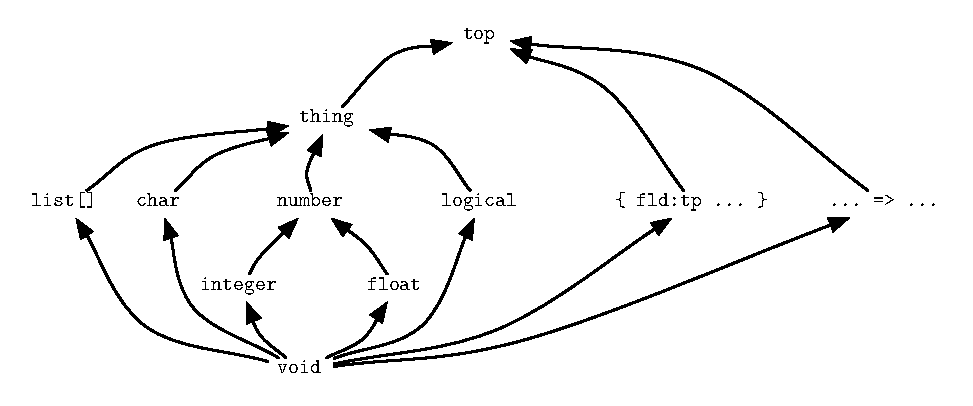
\includegraphics[width=\textwidth]{lattice}}
\caption{\label{type:lattice}Part of \go's standard type lattice}
\end{figure}

In the sub-type partial ordering, higher in the order means more general and lower in the ordering means more specific. Thus \q{top} type is the most general type (and therefore the least is known about values of type \q{top}) and \q{void} is so specific that there are \emph{no} legal \q{void} values.

The significance of \q{top} and \q{void} is largely technical, however, a function that accepts \q{top} arguments will accept anything and a \q{void} value is acceptable for all functions. On the whole, if you see either \q{top} or \q{void} in a type expression in an error message, you are likely to be in trouble!

You will notice that \go's type lattice is wide and shallow -- that for the most part there are few significant \firstterm{chain}{A chain is a sequence of types where for each pair of types in the link \emph{T\subi} and \emph{T\sub{i+1}} it  known that \emph{T\subi} is a subtype of \emph{T\sub{i+1}}. All types are in a chain of at least three elements: \q{void}, the type itself and \q{top}.}s in the lattice. This is in the nature of type lattice systems. However, when defining types, particularly in terms of type inheritance, then we do get a richer network. For example, figure~\vref{type:lattice:number} shows the lattice associated with the \q{number} type.

\begin{figure}
\centerline{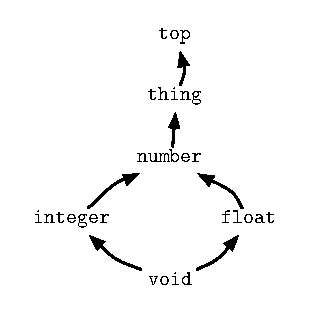
\includegraphics{numberlattice}}
\caption{\label{type:lattice:number}\go's \q{number} type lattice}
\end{figure}

This graph highlights the fact that a lattice is not necessarily a simple \firstterm{basket}{A basket type lattice is one where every chain is exactly three elements long; effectively meaning that there is no significant subtype relationship between non-trivial type elements.} or \emph{chain}, but can have have branching elements in it. It cannot, however, have cycles -- a lattice with a cycle is not permitted.

\subsection{Polymorphism}
Types  may be \firstterm{polymorphic}{A type that is not completely ground -- it may refer to many kinds of values.} and \firstterm{recursive}{A recursive type is one which may have components of the same type as the overall type.}. This polymorphism is reflected in the names of types -- they can have type arguments. For example, the \q{char} type is the type of characters; and \q{list[char]} represents the type list  of \q{char}acters -- i.e., \q{string}s.

The list type (\q{list[\emph{type}]}) is polymorphic: it requires a type argument which is the type of the elements of the list. It is also recursive because the type of a component element of a list term -- namely the tail of the list -- is also of the same type as the whole list.  A recursive type is one whose values contain components that are of the same type as the whole. Although the \q{list[\ldots]} type is built-in to \go, it is straightforward to define new recursive types. 

Recursive types have a particular hallmark: their type terms are \emph{opaque} -- it is not possible to infer solely from the type expression what values of that type look like. For example, although a list is necessarily defined as a term which includes a list as a component (the tail of a list is also a list of the same type) that recursion is not itself reflected in the \q{list} type term. In contrast with this, type expressions for functions are \emph{transparent} -- it is obvious from the type term what the structure of the values are -- and conversely, transparent types may not be recursive. For tuples, that means, for example, that it is not possible to define a tuple type in \go that has the same tuple type as itself as one of the elements of the tuple:
\begin{example}
\begin{boxed}
\begin{alltt}
( number, ( number, ( number, \ldots)))
\end{alltt}
\end{boxed}
\caption{\label{recursive:tuple}an impossible recursive tuple type}
\end{example}

\section{Type inference}
\label{type:inference}

\index{type inference}
\go program expressions are only meaningful if a consistent type assignment or consistent sub-type constraints  can be inferred for them using the declared program and class types. The process of inferring a consistent sent of type assignments and sub-type constraints to a \go program is called \firstterm{type inference}{A process for determining whether a program is type safe or not. A type-unsafe program \emph{might} be able to compute a value, but is likely to not be able to compute a valid value.}.

The fundamental predicate relating types to each other, and hence the key concept for understanding \go's type inference system is the subtype relation. In presenting the sub-type relation we use the notation:
\begin{equation}
\subtype{T\sub{1}}{T\sub2}
\end{equation}
to denote that the type \q{\emph{T\sub1}} is a subtype of \q{\emph{T\sub2}}. Implicit in this is always the possibility that the types \q{\emph{T\sub1}} and \q{\emph{T\sub2}} are \emph{equal}.

As noted above, \go's types form a lattice with more general types being higher in the lattice and more specific types lower in the lattice. 

To define the meaningful type associations we use a form of type inference rule notation. The general form of a type rule is:

\begin{prooftree}
\AxiomC{\mbox{\emph{Condition}}}
\UnaryInfC{\typeprd{E}{X}{T}}
\end{prooftree}
where the intended reading is:
\begin{quote}
The type associated with the expression $X$, in the context of the environment $E$, is $T$ providing that \emph{Condition} holds. Often \emph{Condition} is a conjunction of other type constraints mentioning some of the same variables as in consequent.
\end{quote}
The environment $E$ is a sequence of pairs, of the form \q{(\mbox{\emph{Name}},\mbox{\emph{Type}})}, which is used as a means of recording the type associated with the identifiers that may be in scope when assigning a type.

If we are inferring that one type is less than another, then we are likely to use an inference rule of the form:
\begin{prooftree}
\AxiomC{\mbox{\emph{Condition}}}
\UnaryInfC{\subtype{T\sub{1}}{T\sub2}}
\end{prooftree}
since, in many cases, the subtype inference depends on preconditions being satisfied.

In addition to type associations and subtype determinations, we also need to make certain other kinds of type inference. For example, the \safegoal{E}{Goal} predicate is satisfied if its goal argument is type consistent in environment \emph{E}. Other predicates we will need include \safeact{E}{Act} which is satisfied for an action that is type safe, \grammprd{E}{G}{S} which is satisfied in context $E$ if $G$ is a grammar over streams of type $S$, .

\subsection{Type variables}
The process of type inference is complicated by the fact that it is often not known \emph{what} a particular type actually is. For example, during the inference process associated with the expression:
\begin{alltt}
O.f()
\end{alltt}
the type of \q{O} may not be known immediately. In which case the type inference process will be computing whether
\begin{alltt}
O\sub{t} \impl \{ f:[]=>R\sub{t} \}
\end{alltt}
If the type of \q{O} is not known, then it must record this inequality against the type variable \q{O\sub{t}}; in case another step in the type inference process requires it or other constraints.

In general, in a type lattice, all type variables may be characterized by two types: an upper bound and a lower bound. The upper bound denotes that type which it known that the type variable is \emph{lower} than, and conversely the lower bound determines a \emph{minimum} type for the variable.

The type inference system goes one step further than this: it assumes that if the only thing known about two type variables is that one is greater than the other, it assumes that they are equal. A consequence of this is that the lower and upper bounds of a type variable are always known to be non-variable.

From a strict mathematical point of view, this is a strong inference that is not sanctioned by lattice theory: it is sound -- in the sense that two such types may indeed be equal -- but not complete, since it is quite possible for there to be a third type \emph{between} the upper and lower types.

However, in practice this is not nearly as big an issue as it might seem. The reason is that the most common situation where variable-variable subtyping arises is in recursive programs. Again, in such situations, the most common scenario is:
\begin{alltt}
V\sub1 \impl V\sub2 \impl \ldots V\sub1
\end{alltt}
I.e., all of the type variables are, in fact equal!

Finally, the effect of this restriction is safe; in the sense that potentially type correct programs will be rejected -- but it will not permit a type incorrect program to be accepted. Such false rejections can normally be resolved by additional type annotations on the text of the program that eliminate the implicit uncertainty.

The benefits of this form of type inference are two-fold: the type inference procedure itself is highly efficient and always terminates; and, in the case of erroneous programs, the error messages displayed by the type inference system are bounded.\footnote{Both of these are serious concerns for non-trivial programs.}

\section{Standard Types}
\label{types:types}
\index{types}
\go has a range of built-in `atomic' types:  \q{integer}, \q{float}, \q{char} and \q{symbol}; and a range of built-in \emph{type constructors}:
\begin{itemize}
\item
\q{list[\emph{type}]} (list of \emph{type}), 
\item
\q{[\emph{type\sub1},\ldots,\emph{type\subn}]\{\}} (predicate type), 
\item
\q{[\emph{type\sub1},\ldots,\emph{type\subn}]=>}\emph{type} (function type), 
\item
\q{[\emph{type\sub1},\ldots,\emph{type\subn}]-->}\emph{type} (grammar type),
\item
\q{[\emph{type\sub1},\ldots,\emph{type\subn}]*} (action type), and
\item
\q{\{ \emph{field\sub1}:\emph{type\sub1}. \ldots \emph{field\subn}:\emph{type\subn}. \}} (type interface)
\end{itemize}

\subsection{Type variables}
\label{types:standard:variable}

\index{type variable}
\go does not use any special lexical markers to distinguish type variables from other variables, or even other type names -- the scope of the identifier serves to distinguish the cases. An identifier \q{foo} occurring in a type expression will refer to a type name if a type definition for \q{foo} is `in scope'; otherwise it refers to a type variable.

The normal scope rules do not apply for certain of \go's built-in types; for example, the identifier \q{number} (say) is predefined in the language and always refers to the \q{number} type.

\paragraph{Universally quantified types}
\index{unversally qunatified types}
\index{type variable!universal}
A \emph{universally} quantified type is written using the notation:
\begin{alltt}
[s\sub1,\ldots,s\subn]-\emph{Type}
\end{alltt}
this type binds the type variables s\subi{} occurring in the \emph{Type} expression. \go supports nested quantification of type terms: if \emph{Type} contains a type expression that is itself quantified and binds any or all of the \q{s\subi} type variables then the inner occurrences refer to the inner-most quantification.

It is not normally required to manually identify the type variables in a type expression in this way; however, when type expressions are printed (in error messages typically) they will be displayed in fully quantified form.


\subsection{Standard value types}
\label{types:standard}
\index{types!standard types}

Most of \go's standard types are defined in a standard library: \q{go.stdlib}. This library, which also includes a number of utility definitions, is automatically \q{import}ed in every package.\footnote{It is possible, if not advised, to suppress this behavior with a special compiler option.}

\subsubsection{\q{thing} type}
\label{types:standard:thing}

\index{thing@\q{thing} type}
\index{type!thing@\q{thing} type}

The \q{thing} type is the top of the value part of the type lattice -- all values are a sub-type of \q{thing}. It is not the top of the type lattice itself -- that is \q{top}. The program types -- such as function type -- are not a sub-type of \q{thing} -- although they are sub-types of \q{top}.

The \q{thing} type has a simple type interface; it is declared to be:
\begin{alltt}
thing \impl \{ 
  show:[]=>string.
  meta:[]=>meta.
  \}.
\end{alltt}
The \q{show} function is used to compute a printable \q{string} display of a term and \q{meta} is used to compute a meta-term representation of a term. Note that different types of terms may well use different methods for displaying themselves; it is only the \emph{type} of \q{show} that is defined at this juncture.
  

\subsubsection{\q{number} type}\
\label{types:standard:number}

\index{number@\q{number} type}
\index{type! number@\q{number} type}
The \q{number} type symbol is used to denote the union type of integer and floating point values and expressions. The \q{number} type has the definition:
\begin{alltt}
number \impl thing.
\end{alltt}

\subsubsection{\q{integer} type}
\label{types:standard:integer}

\index{integer@\q{integer} type}
\index{type!integer@\q{integer} type}
The \q{integer} type symbol is used to denote the type of integer values and expressions. The \q{integer} type has the definition:
\begin{alltt}
integer \impl number.
\end{alltt}

\subsubsection{\q{float} type}
\label{types:standard:float}

\index{float@\q{float} type}
\index{type! float@\q{float} type}
The \q{float} type symbol is used to denote the type of floating point values and expressions. The \q{float} type has the definition:
\begin{alltt}
float \impl number.
\end{alltt}

\begin{aside}
  Note that there is no subtype relationship between \q{integer}s and \q{float}s. They are, however, both subtypes of the standard type \q{number}.  This can occasional quirks where it is necessary to specifically convert \q{integer} values to \q{float}s using the built-in function \q{n2float}.
\end{aside}

\subsubsection{\q{char} type}
\label{types:standard:char}

\index{char@\q{char} type}
\index{type!char@\q{char} type}
The \q{char} type symbol is used to denote character values and expressions. The \q{char} type has the definition:
\begin{alltt}
char \impl thing.
\end{alltt}

\subsubsection{\q{symbol} type}
\label{types:standard:symbol}
\index{symbol@\q{symbol} type}
\index{type!symbol@\q{symbol} type}

The \q{symbol} type symbol is use to denote symbol values and expressions. Note that this type refers to the `general' class of symbols -- literals of which are written as identifiers surrounded by single quote characters. The other main class of symbols -- those introduced within user-defined type definitions are not covered by this type symbol; and nor are they written with single quotes.

The \q{symbol} type has the definition:
\begin{alltt}
symbol \impl thing.
\end{alltt}


\subsubsection{\q{logical} type}
\label{types:standard:logical}
\index{logical@\q{logical} type}
\index{type!logical@\q{logical} type}

The \q{logical} type is used to denote truth values. Although a standard type, \q{logical} can be defined as a normal user-defined type, using the type definition:
\begin{alltt}
logical ::= true | false.
\end{alltt}

\subsubsection{\q{opaque} type}
\label{types:standard:opaque}
\index{opaque@\q{opaque} type}
\index{type!opaque@\q{opaque} type}
The \q{opaque} type symbol is used to denote certain `internal' values that are managed by the \go system. There is no written notation that corresponds to opaque literal values, and they will never be displayed in normal circumstances.

\subsubsection{\q{meta} type}
\label{types:standard:meta}
\index{meta@\q{meta} type}
\index{type!meta@\q{meta} type}

The \q{meta} type is used to represent a meta-level representation of a term. It is defined using the definition:
\begin{alltt}
meta \impl thing.
\end{alltt}

\subsubsection{Tuple type}
\label{types:standard:tuple}
\index{tuple@\q{,} type}
\index{type!tuple@\q{,} type}

The \q{,} type is used to denote pairs of values. Although a standard type, \q{,} can be defined as though it were a normal user-defined type, using the definition:
\begin{alltt}
(u,v) ::= (u,v).
\end{alltt}
This rather bizarre type definition declares that the tuple type -- denoted by the type term \q{(u,v)} has a single constructor, also \q{(u,v)}. This notation is a slight twist on the normal type notation -- we are using the \q{,} operator as an infix type operator which is not actually permitted in programs.

\subsubsection{\q{list} type}
\label{types:standard:list}

The list type is used to denote lists of values. The list type is written using the notation:
\begin{alltt}
list[\emph{type}]
\end{alltt}
For example, the type expression:
\begin{alltt}
list[char]
\end{alltt}
denotes the type `list of \q{char}'. This is the type assignment given to expressions which are inferred to be lists of \q{char}acter -- including string literals. \go supports the \q{string} synonym for the \q{list[char]} type term.

The \q{list} type has a definition equivalent to:
\begin{alltt}
list[t] \impl thing.
list[t] \impl \{
    head:[]=>t.                -- head of the list
    tail:[]=>list[t].          -- tail of the list
    eof:[]\{\}.                  -- is the list empty
    cons:[t]=>list[t].         -- new list on the front
    tack:[t]=>list[t].         -- new list on the back
    hdtl:[t,list[t]]\{\}.        -- pick off the head and tail
    eq:[list[t]]\{\}.            -- is equal to this list
\}
\end{alltt}

\subsection{Program types}

\subsubsection{Type modes}
\index{type mode}

Program types have argument types that denote the types of arguments to the program. However, the types of arguments are also associated with \emph{modes} -- which express constraints on the flow of information into or out of a program via its arguments.

There are four kinds of modes: input mode, super-input mode, output mode and bidirectional mode:
\begin{description}
\item[input mode]
If an argument is marked as being input mode then the expectation is that data flows into the program through that argument. This carries two implications: one for type checking and one dynamic data flow:
\begin{itemize}
\item
An actual argument to a program that corresponds to an input moded argument may have a type that is a sub-type of the expected type.
\item
An actual argument to a program must not be \emph{bound} as a result of the matching of input arguments to patterns. Where the actual argument is a non-variable, this is not an issue; where the actual argument is an unbound variable then either the matching pattern also corresponds to an unbound variable or the match will \emph{fail}.
\item
In order to explicitly note an argument type to be input, suffix the type of the argument with the \q{+} operator:
\begin{alltt}
pp:[integer+]\{\}
\end{alltt}
\end{itemize}

\item[super input mode]
The super input mode is based on the input mode; with the additional operational characteristic that if a program is invoked where the super input moded argument is unbound then the call to the program is \emph{delayed} until such time as the variable becomes bound.

If the variable is never instantiated, then the delayed program is never invoked.

The super input mode is marked by suffixing the type of the argument with the \q{++} operator:
\begin{alltt}
listOfInt:[list[integer]++]\{\}
\end{alltt}

\item[output mode]
An output moded argument is the converse of an input moded argument:
\begin{itemize}
\item An actual argument's type must be \emph{equal} to the expected type for that program argument.
\item at run-time an actual argument \emph{must} be an unbound variable; otherwise the matching of patterns to values will \emph{fail} even if the corresponding pattern is an unbound variable.
\item
In order to explicitly note an argument type to be output, suffix the type of the argument with the \q{-} operator:
\begin{alltt}
pp:[integer-]\{\}
\end{alltt}
\end{itemize}

\item[bidirectional mode]
A bidirectional moded argument can be either input or output; and unification is used to match the actual argument to the pattern.
\begin{itemize}
\item
The type of the actual argument must be equal to the expected type for that argument
\item
Unification is used to match the incoming value against the pattern; hence the flow of information may be either incoming, outgoing or a mixture.
\item
In order to explicitly note an argument type to be bidirectional, suffix the type of the argument with the \q{-+} operator:
\begin{alltt}
pp:[integer-+]\{\}
\end{alltt}
\end{itemize}
\end{description}

Although it is possible to associate modes with every argument type of every program type, program types have defaults that are intended to represent the normal mode of use for that kind of program.

\subsubsection{Function type}
\label{types:standard:function}

The function type is used to denote function values. The function type is written:
\begin{alltt}
[\emph{T\sub{1}},\ldots,\emph{T\sub{n}}] \funarrow{} \emph{T\sub{R}}
\end{alltt}
where \q{[\emph{T\sub{1}},\ldots,\emph{T\sub{n}}]} is a list of the type expressions corresponding to the arguments of the function and \emph{T\sub{R}} corresponds to the result of the function. For example, the type expression:
\begin{alltt}
[list[char],list[char]]=>list[char]
\end{alltt}
denotes a function -- from two string arguments to a string result.

The default mode for function arguments is \emph{input}. However, it is occasionally useful to mark a function argument as output -- as an out-of-band way of returning values from a function.

\subsubsection{Predicate type}
\label{types:standard:predicate}

The predicate type is used to denote relational or predicate values. The predicate type is written:
\begin{alltt}
[\emph{T\sub{1}},\ldots,\emph{T\sub{n}}]\{\}
\end{alltt}
where \q{[\emph{T\sub{1}},\ldots,\emph{T\sub{n}}]} is the list of type expressions of the arguments of the predicate. For example, the type expression:
\begin{alltt}
[list[char],list[char],list[char]]\{\}
\end{alltt}
denotes the type of a ternary predicate where all the arguments are strings.

The default mode for predicate arguments is \emph{bidirectional}. However, it is often useful to mark a predicate argument as input -- to be explicit about the expect usage of the predicate.


\subsubsection{Action type}
\label{types:standard:action}

The action type is used to denote procedure values. The action type is written using a postfix \q{*} operator:
\begin{alltt}
[\emph{T\sub{1}},\ldots,\emph{T\sub{n}}]*
\end{alltt}
where \q{[\emph{T\sub{1}},\ldots,\emph{T\sub{n}}]} is the list of type expressions of the arguments of the procedure. For example, the type expression:
\begin{alltt}
[list[char]]*
\end{alltt}
denotes the type of a unary procedure whose single argument is a string.

The default mode for action procedure arguments is \emph{input}. However, it is occasionally useful to mark an argument as output -- as that is the only way of arranging for output from an action procedure call.

\subsubsection{Grammar type}
\label{types:standard:grammar}

The grammar type is used to denote grammar values. The grammar type is written as a \q{-->} mapping from the types of the arguments of the grammar to the type of the stream of values the grammar is defined over:
\begin{alltt}
[\emph{T\sub{1}},\ldots,\emph{T\sub{n}}] --> \emph{T\sub{S}}
\end{alltt}
where \q{[\emph{T\sub{1}},\ldots,\emph{T\sub{n}}]} is the list of type expressions of the arguments of the grammar and \emph{T\sub{S}} is the type of the stream that the grammar is defined over -- typically a list of some kind. For example, the type expression:
\begin{alltt}
[number]-->list[char]
\end{alltt}
denotes the type of a grammar whose single argument is a number and which may be used to parse strings.

The default mode for grammar arguments is \emph{bidirectional}. However, it is occasionally useful to mark a grammar argument as input -- to be explicit about the expect usage of the grammar, and also to mark an argument as output -- to be explicit about the outputs associated with parsing a stream.

\subsubsection{Class type}
\label{types:standard:class}

\index{type!class}
\index{class type}
\index{type!@= type operator}
There are two kinds of class type declarations: those that introduce a stateless class and those that introduce a stateful class.

The state-free class type is used to denote constructor classes, analogous to constructor functions. The stateful class type denotes classes that may carry state.


A state-free class type declaration takes the form:
\begin{alltt}
\emph{class}:[\emph{T\sub1},\ldots,\emph{T\subn}] @= \emph{Type}.
\end{alltt}
The only permitted mode for the label arguments of a state-free class label is \emph{bidrectional}.

A stateful class type declaration takes the form:
\begin{alltt}
\emph{class}:[\emph{T\sub1},\ldots,\emph{T\subn}] @> \emph{Type}.
\end{alltt}
The default mode for label arguments of a stateful class label is \emph{input}.

\begin{aside}
The reason that state-free label arguments must be bi-directional is that class labels are equivalent to constructor functions: i.e., they have an inverse. That means that it is always possible to recover the arguments of a 'call' to a constructor function.

On the other hand, one of the differences between state-free class labels and statefull class labels is that the latter \emph{do not} have inverses -- they are semantically closer to regular functions.
\end{aside}
Note that a class type statement does not define the class itself, it simply defines its type.

\section{Algebraic type definitions}
\label{type:algebraic}

In addition to a type being defined using the sub-type statements, a type may also be introduced using an \emph{algebraic type definition} statement. An algebraic type definition is one where the type is introduced at the same time as a set of enumerated symbols and constructors for the type:
\begin{alltt}
\emph{UserT}[\emph{T}\sub1,\dots,\emph{T}\subn] ::= \dots\ | \emph{S} | \dots.
\end{alltt}
where \emph{T\subi} are identifiers indicating type arguments and the right hand side is a series of enumerated symbols and constructor function templates.

For example, the \q{tree} type defined below may be used to denote tree values:

\begin{alltt}
tree[a] ::= empty | node(tree[a],a,tree[a]).
\end{alltt}
This statement defines a new type type constructor \q{tree} together with the enumerated symbols and constructor terms that make up values of the \q{tree} type.

\subsection{Type parameters of a type definition}
\label{type:parameter}

Where the template of a \emph{UserType} takes the form:
\begin{alltt}
\emph{UserType}[\emph{T}\sub1,\dots,\emph{T}\subn] \impl \ldots
\end{alltt}
the various arguments \emph{T\subi} are the \emph{type parameter}s of the type definition. They must all be identifiers and they are interpreted as type variables. Such a \emph{UserType} is implicitly universally quantified with respect to the type parameters (hence the polymorphism of the type).

\go imposes a restriction on type variables occurring in a type definition: all type variables appearing in the body of the type definition -- i.e., appearing in templates for the type constructors in class definitions -- must also appear in the type template expression itself.

\subsection{Enumerated symbol}
\label{type:user-symbol}
An \emph{enumerated} symbol is equivalent to a zero-arity label term. For example, the introduction of \q{empty} in the definition of \q{tree} above is equivalent to the class definition:
\begin{alltt}
empty:tree[a] .. \{\}.
\end{alltt}

The type analysis of a definition of an enumerated symbol may be captured via an `introduced' type inference rule:
\begin{equation*}
\forall \vec{V}.\left\{\frac{}
{\typeprd{E}{\q{S}}{\q{\emph{UserT}[\emph{T}\sub1,\dots,\emph{T}\subn]}}}\right\}
\end{equation*}
where $\vec{V}$ are all the type variables ocurring in the type definition and \q{S} is the newly introduced enumerated symbol.

Note that, in general, the type of a enumerated symbol can have type variables even when clearly the symbol itself has no variables. We can see this more clearly with the empty list case. \go's list notation is based on the \q{,..} constructor function and the \q{[]} enumerated symbol; which might be captured in the algebraic type definition:
\begin{alltt}
list[T] ::= [T,..list[T]] | []
\end{alltt}
The type of an occurrence of the empty list is, then, an expression of the form:
\begin{alltt}
list[T\sub{i}]
\end{alltt}
where \q{T\sub{i}} may or may not be known. The logic of this is that an empty list is always of a list of a specific type -- even if we cannot determine what that type is in given circumstances.

\subsection{Constructor functions}
\label{type:constructor}
\index{contructor function definition}
\index{functions!constructor}

Constructor functions (a.k.a. class labels) are analogous to functors in \prolog: they fulfill very similar roles. However, their semantics are quite distinct to normal \prolog terms since they always are associated with logical theories -- even when defined within an algebraice type definition.

\begin{aside}
  Constructor functions are so-named because they are functions: with the
  particular property that every expression involving the constructor function
  has an exact inverse. This property allows constructor functions to be used as
  patterns as well as in other expressions.
\end{aside}

The type assignment for constructor functions can be viewed as an additional type inference rule; where a type definition was of the form:
\begin{alltt}
\emph{Template} ::= \ldots | \emph{F}(\emph{T\sub1},\ldots,\emph{T\subn}) | \ldots
\end{alltt}
we introduce a new inference rule of the form:
\begin{equation}
\LeftLabel{$\forall \vec{V}$}
\AxiomC{\typeprd{{\emph{E}}}{A\sub1}{\emph{T\sub{1}}}}
\AxiomC{\ldots}
\AxiomC{\typeprd{{\emph{E}}}{A\subn}{\emph{T\sub{n}}}}
\TrinaryInfC{\typeprd{{\emph{E}}}{\q{\emph{F}(\emph{A\sub1},\ldots,\emph{A\subn})}}
{\q{\emph{Template}}}}
\DisplayProof
\end{equation}
where $\vec{V}$ are the type variables ocurring in the type definition.

\subsection{Type extension}
One of the key features of \go's type system is its extensibility. In particular, because types are distinct from classes, there is always the potential to introduce new constructors for a type -- including types that have been introduced using an algebraic type definition.

For example, given the \q{tree[]} type, we may decide that we need a new kind of node for a tree -- perhaps a binary tree node that does not include a label. We can do so simply by defining a class for it:
\begin{alltt}
bin:[tree[a],tree[a]]@=tree[a].
bin(L,R) .. \{ \ldots \}
\end{alltt}
The effect of this is as though the original type definition were:
\begin{alltt}
tree[a] ::= empty 
        | node(tree[a],a,tree[a])
        | bin(tree[a],tree[a]).
\end{alltt}
We can even introduce this class in a different package than the one in which \q{tree[]} itself is defined:
\begin{alltt}
foo\{
  import tree.
  bin:[tree[a],tree[a]]@=tree[a].
  bin(L,R) .. \{ \ldots \}
\}
\end{alltt}
  

